\begin{frame}{Existence of Featureless Insulators}
\vskip-1.5cm
\only<1>{
\begin{block}{
Status of existence question:}
\bi 
\item On {\em non-symmorphic} lattices, not all integer particle-numbers can be realized.
\bi 
\item Flux removal doesn't commute with glide-reflections or screw-axes where the the translation vector is not a lattice translation.
\ei 
\note{Lieb-Schultz-Mattis extended again: $(J - m)/S$ must be integer.}

\item On Kagome lattice, boson insulator with 1/3 site filling constructed by filling Wannier orbitals of the lowest band of a fermion band insulator. 
\begin{figure}
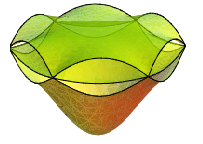
\includegraphics{diagrams/kagomeband.png}
\end{figure}
\ei 
\end{block}
}
\only<2>
{
On honeycomb lattice, no such band insulator. 
\bi 
\item Proposed wavefunction:
$$
\ket{\psi} = \prod\limits_R \sum\limits_{i \in R} b^{\dagger}_i \ket{\vec{0}}
$$
\item Goals:
\bi 
\item Rule out spontaneous symmetry breaking by computing correlations
\item Rule out topological order by computing topological entanglement entropy
\item Distinguish from other featureless phases using edge entanglement
\ei 
\ei 
}
\end{frame}